Early approaches to inferring cosmological parameters from time delay
lens observations focused on measuring the Hubble constant in a
Friedman-Robertson-Walker model with asserted (fixed) density
parameters.\footnote{The original investigation by \citet{Ref64}
involved the ``assumption that the linear distance--red-shift relation
is valid.''} With better data came the recognition that time delay
lenses were really probes of cosmological distance
\citep{Koo++03,Suy++10}, and the emphasis shifted to
inferring the set of cosmological parameters that are needed to predict
the kinematics of the expansion of the Universe out to the redshift of
the source.
The parameter most strongly constrained is still the Hubble constant,
but as sample sizes increase we expect ensembles of lenses to support
the inference of several cosmological parameters \citep[or combinations
thereof][]{LewisAndIbata2002}.

In Figure~\ref{fig:current-constraints} we reproduce the current
constraints on cosmological parameters, from the two best-measured
systems, B1608$+$656 and RXJ1131 \citep{Suy++14}. When this figure was
made, the available precision from just these two lenses was about the
same as that from SDSS DR7 Baryonic Acoustic Oscillations
\citep{PercivalEtal2010} or the ``Constitution'' set of Type Ia
supernovae \citep{HickenEtal2009}.  When all three of the curvature
density $\Ok$, Dark Energy density $\ODE$ and equation of state $\wDE$
parameters are allowed to vary, along with $H_0$, we see that the time
delay lenses provide similar constraints to BAO and complementary
constraints to the SNe: the time delays and the BAO signal depend on
angular diameter distances and $H_0$, while the supernovae probe
relative luminosity distances.

%%%%%%%%%%%%%%%%%%%%%%%%%%%%%%%%%
\begin{figure*}[!ht]
\centering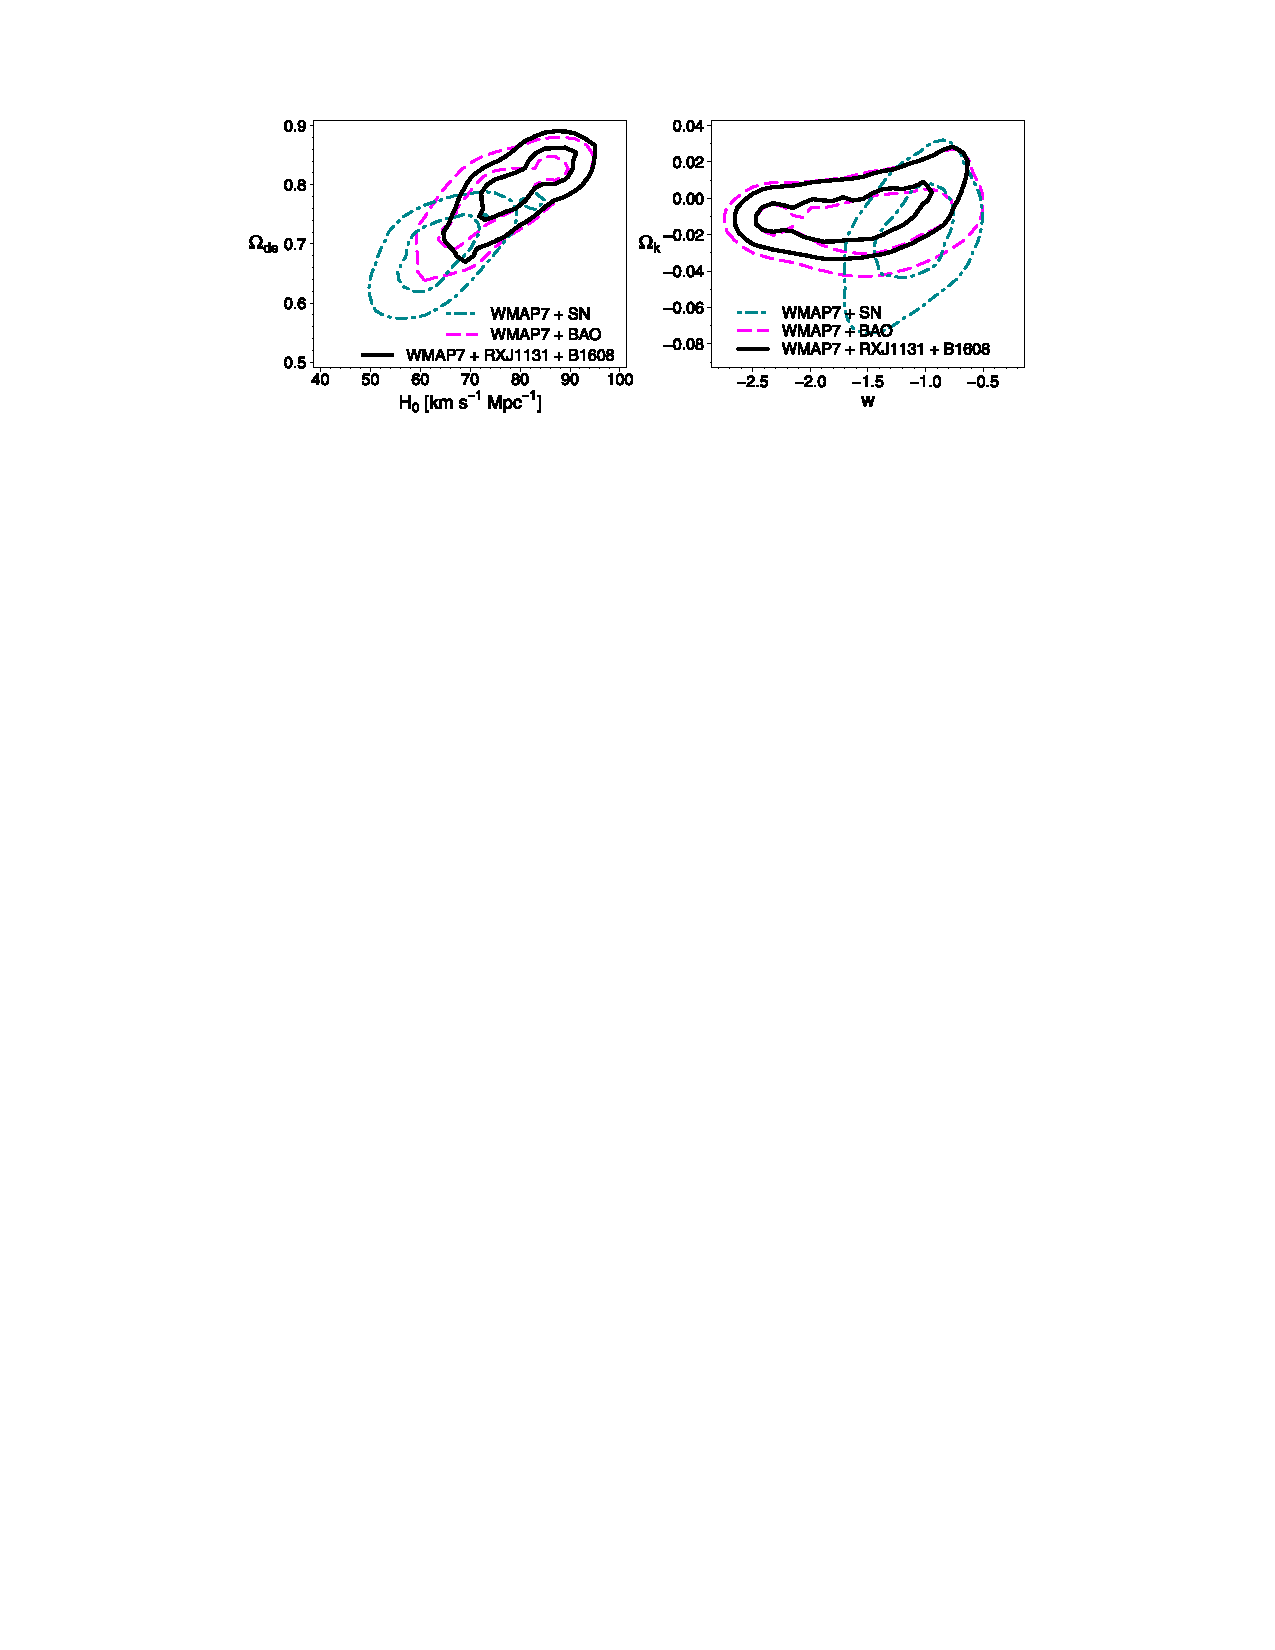
\includegraphics[width=0.9\linewidth]{figures/Suyu13_fig11.pdf}
\caption{Cosmological parameter constraints from time delay
lenses \citep{Suy++13}. The marginalized posterior PDFs, given the combined B1608$+$656
and RXJ1131 datasets and the assumption of an open CDM cosmology with
unknown dark energy equation of state, are shown in
two sets of two parameter dimensions,
and compared to those given contemporary BAO and Type Ia supernova data.
Image reproduced with permission from \citet{Suy++13}, copyright by AAS.}
\label{fig:current-constraints}
\end{figure*}
%%%%%%%%%%%%%%%%%%%%%%%%%%%%%%%%%

One important feature of the cosmological parameter inference carried
out in the RXJ1131 analysis of \citet{Suy++13} is that it was blinded.
Following the simple methodology suggested in the blind Type Ia
supernova analysis of \citet{Con++06}, all cosmological parameter PDFs
were plotted with centroids offset to the origin until the team agreed
(after notably lengthy discussions about systematic errors) to ``open
the box,'' just before publication.\footnote{Importantly, the authors
agreed to publish the unblinded results, no matter what.} Such
attempts to avoid ``unconscious experimenter bias'' introduced by
stopping systematics analysis when the ``right answer'' is obtained
have long been advocated in particle physics
\citep{klein2005blind}, and seem likely to become the standard in
cosmology as well \citep[e.g.][]{STEP,DESWL}. It is also crucial to
repeat the measurements using independent codes, assumptions, and
techniques, in order to quantify associated systematic
uncertainties. It is re-assuring that the independent analysis of
RXJ1131 carried by out by \citet{BAR16}, the one based on
more flexible models carried out by \citet{Suy++14}, and the one based
on ground based adaptive optics data by \citet{Che++16} find results that are
statistically consistent with the original blind analysis \citep{Suy++13}.

While the sample of very well-measured lenses was being painstakingly
expanded from zero to two, the exploration of statistical approaches
to dealing with large samples of lenses began.  Compressing the image
configuration and time delay in double image systems into a single
summary statistic, \citet{Ogu07b} derived a scaleable method for
measuring the Hubble constant (but not the other cosmological
parameters) from samples of lenses, finding
$H_0=68\pm6\,{\rm(stat.)}\,\pm8\,{\rm (syst.)}\,{\rm km s}^{-1}{\rm
Mpc}^{-1}$ from a sample of 16 lenses with measured time delays. The
systematic uncertainties associated with this result may be hard to
reduce given the approximations made: while the summary statistic is
model-independent, the interpretation is not.

An alternative approach is to work with more flexible lens models, fit
the data for each one, and combine the whole sample in a joint
inference.  This is the approach taken by \citet{Sah++06}, who found
$72^{+8}_{-11}\,{\rm km s}^{-1}{\rm Mpc}^{-1}$ from 10 lenses (again
assuming fixed curvature and dark energy parameters).
The amount of
information system used in this analysis was minimal: only the quasar
positions and time delays were taken as inputs. The high flexibility of the free
form models employed led to a likelihood that was effectively identically 1 or 0, and thus the
results are dominated by prior constraints set on the pixels and their
regularization \cite[see][for a description of pixel-lens in Bayesian
terms]{Col08}. Specifically, the known physical degeneracy between
density profile slope and predicted time delay
\citep{Wuc02,Suyu12} is broken by the choice of pixel value prior probability
distribution function. This assumption was tested by
\citet{Rea++07}, who used a hydrodynamic simulation of an elliptical
galaxy to generate mock image position and time delay data, and
confirm the accuracy of the previous study's Hubble constant
uncertainties. With improved time delay estimates in larger samples of
lenses, \cite{P+J10} and then \citet{RK++2015} reduced the random
uncertainty further.

While focused only on the Hubble constant and carried out unblind, and
with the lens environment and line of sight mass structures remain
unaccounted for and further tests on realistic simulated galaxies
warranted, these ensemble studies point the way towards a future of
considerably larger sample sizes. Our aspirations towards high accuracy
demand that we adopt more flexible mass models and then
cope with the degeneracies;
it is clear that such large
scale analysis will need careful consideration of the choice of the
priors, and ideally the ability to use more information than just the
image positions and time delays. We discuss these issues in detail in
the next section.
